%% LyX 2.3.2-1 created this file.  For more info, see http://www.lyx.org/.
%% Do not edit unless you really know what you are doing.
\documentclass[english]{article}
\usepackage[T1]{fontenc}
\usepackage[latin9]{luainputenc}
\usepackage{babel}
\usepackage{array}
\usepackage{textcomp}
\usepackage{amsmath}
\usepackage{graphicx}
\usepackage[unicode=true]
 {hyperref}

\makeatletter

%%%%%%%%%%%%%%%%%%%%%%%%%%%%%% LyX specific LaTeX commands.
%% Because html converters don't know tabularnewline
\providecommand{\tabularnewline}{\\}

\makeatother

\begin{document}
\title{Chapter 7: Chi-square Test}
\maketitle

\section{Example}
\begin{enumerate}
\item $H_{0}:$ The die is fair $\left(p=\frac{1}{6}\right)$
\item $H_{1}:$ The die is unfair $\left(p\neq\frac{1}{6}\right)$
\item At $\alpha=0.05$, critical value = $\chi_{\alpha;m-t-1}^{2}$.
\item ~
\begin{align*}
\chi_{0.05;6-0-1}^{2} & =\chi_{0.05;5}^{2}\\
 & =11.070
\end{align*}
\item Rejection region: (remember Chi-square distribution does NOT have
a negative region)
\[
\chi^{2}>11.07
\]
\item %
\begin{tabular}{|c|c|c|c|c|c|c|c|}
\hline 
Number & 1 & 2 & 3 & 4 & 5 & 6 & Total\tabularnewline
\hline 
\hline 
$O_{i}$ & 89 & 113 & 98 & 104 & 117 & 79 & 600\tabularnewline
\hline 
$E_{i}$ & 100 & 100 & 100 & 100 & 100 & 100 & 600\tabularnewline
\hline 
$O_{i}-E_{i}$ & -11 & 13 & -2 & -4 & 17 & -21 & \tabularnewline
\hline 
$\left(O_{i}-E_{i}\right)^{2}$ & 121 & 169 & 4 & 16 & 289 & 441 & \tabularnewline
\hline 
$\frac{\left(O_{i}-E_{i}\right)^{2}}{E_{i}}$ & 1.21 & 1.69 & 0.04 & 0.16 & 2.89 & 4.41 & 10.40\tabularnewline
\hline 
\end{tabular}
\item Since $\chi^{2}=10.40<11.07$, we failed to reject $H_{0}$ at 5\%
significance level. Hence, we do not have enough evidence to conclude
that the observed frequencies are significantly different from those
expected of a fair die.
\end{enumerate}

\section{Example}

Since every city have equal sales potential, therefore, each sale
should be $\frac{\sum x}{n}$, which is the mean.
\begin{enumerate}
\item Hypothesis
\begin{enumerate}
\item Claim: Each of the seven cities have equal sales potential. $\left(H_{0}\right)$
\item Opposite: Each of the seven cities do not have equal sales potential.
$\left(H_{1}\right)$
\item $H_{0}:A=B=C=D=E=F=G$
\item $H_{1}:A\neq B\neq C\neq D\neq E\neq F\neq G$
\end{enumerate}
\item Find the critical value
\begin{enumerate}
\item $\alpha=0.05$
\item $\chi_{0.05;7-1}^{2}=\chi_{0.05;6}^{2}=12.592$
\end{enumerate}
\item Find the rejection region
\begin{enumerate}
\item $\chi^{2}>12.592$
\end{enumerate}
\item %
\begin{tabular}{|c|c|c|c|c|c|c|c|c|}
\hline 
City & A & B & C & D & E & F & G & Total\tabularnewline
\hline 
\hline 
$O_{i}$ & 120 & 185 & 260 & 190 & 210 & 175 & 260 & \tabularnewline
\hline 
$E_{i}$ & 200 & 200 & 200 & 200 & 200 & 200 & 200 & 1400\tabularnewline
\hline 
$\frac{\left(O_{i}-E_{i}\right)^{2}}{E_{i}}$ & $\frac{\left(120-200\right)^{2}}{200}=32$ & $\frac{\left(185-200\right)^{2}}{200}=1.125$ & $\frac{\left(260-200\right)^{2}}{200}=18$ & $\frac{\left(190-200\right)^{2}}{200}=0.5$ & $\frac{\left(210-200\right)^{2}}{200}=0.5$ & $\frac{\left(175-200\right)^{2}}{200}=3.125$ & $\frac{\left(260-200\right)^{2}}{200}=18$ & 73.25\tabularnewline
\hline 
\end{tabular}
\item Since $\chi^{2}=73.25>12.592$, we reject $H_{0}$and do not have
enough evidence to conclude that each of the seven cities have equal
sales potential.
\end{enumerate}

\section{Example}
\begin{enumerate}
\item Hypothesis
\begin{enumerate}
\item Claim: The local hospital follows the national pattern. $\left(H_{0}\right)$
\item Oppo: The local hospital do not follow the national pattern. $\left(H_{1}\right)$
\end{enumerate}
\item Find the rejection region
\begin{enumerate}
\item $\alpha=0.05$
\item $\chi_{0.05;7-1}^{2}=\chi_{0.05;6}^{2}=12.592$
\item Rejection region: $\chi^{2}>12.592$
\end{enumerate}
\item Find the Chi-square score
\item %
\begin{tabular}{|c|c|c|c|c|c|c|c|c|}
\hline 
Number of times admitted & 1 & 2 & 3 & 4 & 5 & 6 & 7 & Total\tabularnewline
\hline 
\hline 
$O_{i}$ & 165 & 79 & 50 & 44 & 32 & 20 & 10 & 400\tabularnewline
\hline 
$E_{i}$ & 400{*}40\%=160 & 80 & 56 & 40 & 32 & 24 & 8 & \tabularnewline
\hline 
$\frac{\left(O_{i}-E_{i}\right)^{2}}{E_{i}}$ & $\frac{\left(165-160\right)^{2}}{160}$ & $\frac{\left(79-80\right)^{2}}{80}$ & $\frac{\left(50-56\right)^{2}}{56}$ & $\frac{\left(44-40\right)^{2}}{40}$ & $\frac{\left(32-32\right)^{2}}{32}$ & $\frac{\left(20-24\right)^{2}}{24}$ & $\frac{\left(10-8\right)^{2}}{8}$ & 2.378\tabularnewline
\hline 
\end{tabular}
\item Since $\chi^{2}=2.378<12.592$, we failed to reject $H_{0}$. Hence,
we conclude that the local hospital follows the national pattern.
\end{enumerate}

\section{Example}
\begin{enumerate}
\item Hypothesis
\begin{enumerate}
\item Claim: The results support the theory $\left(H_{0}\right)$
\item Opposite: The results do not support the theory $\left(H_{1}\right)$
\end{enumerate}
\item Find the rejection region
\begin{enumerate}
\item $\chi_{0.05;3-1}^{2}=5.991$
\item $\chi^{2}>5.991$
\end{enumerate}
\item Calculate the Chi-score
\begin{enumerate}
\item %
\begin{tabular}{|c|c|c|c|c|}
\hline 
Color & $O_{i}$ & $E_{i}$ & $\frac{\left(O_{i}-E_{i}\right)^{2}}{E_{i}}$ & \tabularnewline
\hline 
\hline 
Red & 84 & 83.25 & 0.00676 & \tabularnewline
\hline 
Blue & 92 & 83.25 & 0.91967 & \tabularnewline
\hline 
Purple & 157 & 166.5 & 0.54204 & \tabularnewline
\hline 
 & 333 &  & 1.46847 & \tabularnewline
\hline 
\end{tabular}
\end{enumerate}
\item $\chi^{2}=1.46847<5.991$. We failed to reject $H_{0}$ at $\alpha=0.05$
and conclude that the result support the genetic theory.
\end{enumerate}

\section{Example}
\begin{enumerate}
\item Hypothesis
\begin{enumerate}
\item Claim: The random number generator is working incorrectly. $H_{1}$
\item Hypo: The random number generator is working correctly. $H_{0}$
\end{enumerate}
\item The critical value
\begin{enumerate}
\item $\chi_{0.05;6-1}^{2}=11.070$
\item Rejection region: $\chi^{2}>11.070$
\end{enumerate}
\item Find the test statistic
\begin{enumerate}
\item %
\begin{tabular}{|c|c|c|c|c|}
\hline 
Interval & $O_{i}$ & Probability, $P_{i}$ & $E_{i}=500*P_{i}$ & $\frac{\left(O_{i}-E_{i}\right)^{2}}{E_{i}}$\tabularnewline
\hline 
\hline 
$s<4$ & 10 & $P\left(Z<\frac{4-6}{1}\right)=P\left(Z<\text{\textminus}2\right)=0.02275$ & 11.375 & 0.16621\tabularnewline
\hline 
$4\le s<5$ & 75 & 0.13595 & 67.975 & 0.74601\tabularnewline
\hline 
$5\le s<6$ & 163 & 0.34130 & 170.65 & 0.34294\tabularnewline
\hline 
$6\le s<7$ & 174 & 0.34130 & 170.65 & 0.06576\tabularnewline
\hline 
$7\le s<8$ & 66 & 0.13595 & 67.975 & 0.05738\tabularnewline
\hline 
$s\ge8$ & 12 & 0.02285 & 11.375 & 0.3434\tabularnewline
\hline 
Total &  & 1.0000 & 500 & \textbf{1.39264}\tabularnewline
\hline 
\end{tabular}
\item Note: For the probability, use the Z-score
\[
P\left(s>\bar{x}\right)=P\left(Z>\frac{\bar{x}-\mu}{\sigma}\right)
\]
\item Use \href{http://onlinestatbook.com/2/calculators/normal_dist.html}{Normal Distribution Calculator from OnlineStatBook}
to quickly calculate without converting to normal.
\end{enumerate}
\item Conclusion
\begin{enumerate}
\item Since $\chi_{2}=1.39264<11.070$, we failed to reject $H_{0}$, and
hence conclude that the random number generator is working correctly.
\end{enumerate}
\end{enumerate}

\section{Example}
\begin{enumerate}
\item Hypothesis
\begin{enumerate}
\item Claim: The distribution of X is $B\left(3,0.25\right)$ $\left(H_{0}\right)$
\item Oppo: The distribution of X is not $B\left(3,0.25\right)$ $\left(H_{1}\right)$
\end{enumerate}
\item Find the critical value
\[
\alpha=0.01
\]

\begin{enumerate}
\item Critical value
\begin{align*}
\chi_{\alpha;m-t-1}^{2} & =\chi_{0.01;3-0-1}^{2}\\
 & =\chi_{0.01;2}^{2}\\
 & =9.210
\end{align*}
\end{enumerate}
\item Rejection region
\[
\chi^{2}>9.210
\]

\begin{enumerate}
\item If this is true, the probability distribution of X is 
\[
P\left(X=x\right)=^{3}C_{x}\left(0.25\right)^{x}0.75^{3-x}
\]
\end{enumerate}
\item %
\begin{tabular}{|c|c|c|c|c|c|}
\hline 
X & $O_{i}$ & Probability, $p_{i}$ & $E_{i}=64p_{i}$ & $\frac{\left(O_{i}-E_{i}\right)^{2}}{E_{i}}$ & Total\tabularnewline
\hline 
\hline 
0 & 21 & $\frac{21}{21+31+12+0}=0.4219$ & 27 & 1.333 & \tabularnewline
\hline 
1 & 31 & 0.4219 & 27 & 0.5926 & \tabularnewline
\hline 
2,3 & 12 & 0.1563 & 10 & 0.4 & 2.3259\tabularnewline
\hline 
\end{tabular}
\begin{enumerate}
\item $p_{0}=^{3}C_{0}*\left(0.25\right)^{0}*\left(0.75\right)^{3}=0.4219$
\item $p_{1}=^{3}C_{1}*\left(0.25\right)^{1}*\left(0.75\right)^{2}=0.4219$
\item $p_{2+3}=^{3}C_{2}*\left(0.25\right)^{2}*\left(0.75\right)^{1}+{}^{3}C_{3}*\left(0.25\right)^{3}=0.1563$
\end{enumerate}
\item Since $\chi^{2}=2.3259<9.210.$ We failed to reject $H_{0}$, and
hence do not have enough evidence to show that the recorded data do
not fit $B\left(3,0.25\right)$.
\end{enumerate}

\section{Example}

Note: We should not round it from 2.02 to 2.00, oterhwise it will
be inaccurate during exams.

\section{Example}

\subsection{Extra Notes}

By following the probability multiplication rule, if they are independent,
the expected frequency for a field in a two-way table will be
\begin{enumerate}
\item Proportion probability of something happening in the row, multiple
by the proportion probability of something happening in a column (to
get row {*} column proportion) and then multipled by the sample size.
\item Eg:
\[
1000\left(sample\right)*\left(\frac{100}{1000}\left(row\right)*\frac{100}{1000}\left(column\right)\right)=10\left(expected\right)
\]
\end{enumerate}

\subsection{Example}
\begin{enumerate}
\item Hypothesis
\begin{enumerate}
\item The number of accidents depend on the visits by the inspector. $\left(H_{0}\right)$
\item The number of accidents do not depend on the visits by the inspector.
$\left(H_{1}\right)$
\end{enumerate}
\item Critical value
\begin{align*}
\chi_{0.05;\left(4-1\right)\left(2-1\right)}^{2} & =\chi_{0.05;3}^{2}\\
 & =7.815
\end{align*}

\begin{enumerate}
\item Note : $D.O.F.=\left(Row-1\right)\left(Column-1\right)$
\item ~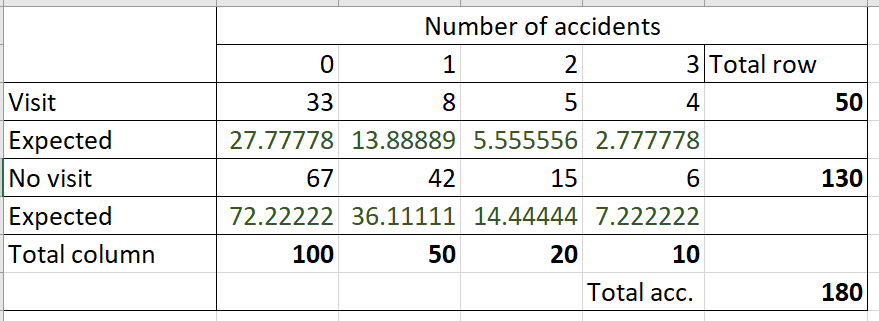
\includegraphics[width=0.8\paperwidth,height=0.8\textheight,keepaspectratio]{lyx-img/c7q8expected}
\end{enumerate}
\item Rejection region
\[
\chi^{2}>7.815
\]
\item Find the test-statistic
\begin{align*}
\chi^{2} & =\frac{\left(33-27.778\right)^{2}}{27.778}+\frac{\left(8-13.889\right)^{2}}{13.889}+\frac{\left(5-5.556\right)^{2}}{5.556}+\frac{\left(4-2.778\right)^{2}}{5.556}+\frac{\left(67-72.222\right)^{2}}{72.222}+\frac{\left(42-36.111\right)^{2}}{36.111}+\frac{\left(15-14.444\right)^{2}}{14.444}+\frac{\left(6-7.222\right)^{2}}{7.222}\\
 & =5.3692
\end{align*}
\item Conclusion
\begin{enumerate}
\item Since $\chi^{2}=5.3692<7.815$. We failed to reject $H_{0}$, and
hence do not have enough evidence to conclude that the number of accidents
do not depend on the visits by the inspector.
\end{enumerate}
\end{enumerate}

\section{Example}

\section{Example}
\begin{enumerate}
\item Hypothesis
\begin{enumerate}
\item Hypo: The coin is fair $\left(H_{1}\right)$
\item Oppo: The coin is unfair $\left(H_{0}\right)$
\end{enumerate}
\item Critical value at $\alpha=0.05$
\begin{enumerate}
\item Critical value: $\chi_{0.05;2-0-1}^{2}=\chi_{0.05;1}^{2}=3.841$
\end{enumerate}
\item Rejection range: $\chi^{2}>3.841$
\item Test-statistics
\begin{align*}
\chi^{2} & =\sum_{i=1}^{m}\frac{\left(\left|O_{i}-E_{i}\right|-0.5\right)^{2}}{E_{i}}\\
 & =\frac{\left(\left|115-100\right|-0.5\right)^{2}}{100}+\frac{\left(\left|85-100\right|-0.5\right)^{2}}{100}\\
 & =4.205
\end{align*}
\end{enumerate}

\section{Example}
\begin{enumerate}
\item Hypothesis
\begin{enumerate}
\item $\left(H_{0}\right)$ There is no association between taking the new
drug and attack by the disease
\item $\left(H_{1}\right)$ There is an association between taking the new
drug and attack by the disease
\end{enumerate}
\item Critical value
\begin{enumerate}
\item $\chi_{0.05;\left(2-1\right)\left(2-1\right)}^{2}=\chi_{0.05;1}^{2}=3.841$
\end{enumerate}
\item Rejection range
\begin{enumerate}
\item $\chi^{2}>3.841$
\end{enumerate}
\item Test-statistic (apply Yate's correction because $D.O.F.=1$)
\begin{enumerate}
\item ~%
\begin{tabular}{|>{\centering}p{0.8\textwidth}|c|c|c|}
\hline 
 & Drugged & Drugless & Total row\tabularnewline
\hline 
\hline 
Attacked & 24 & 32 & 56\tabularnewline
\hline 
Expected & (35.47) & (20.53) & \tabularnewline
\hline 
Not attacked & 52 & 12 & 64\tabularnewline
\hline 
Expected & (40.53) & (23.47) & \tabularnewline
\hline 
Total column & 76 & 44 & 120\tabularnewline
\hline 
\end{tabular}
\item $\chi^{2}=\frac{\left(\left|24-35.47\right|-0.5\right)^{2}}{35.47}+\frac{\left(\left|32-20.53\right|-0.5\right)^{2}}{20.53}+\frac{\left(\left|52-40.53\right|-0.5\right)^{2}}{40.53}+\frac{\left(\left|12-23.47\right|-0.5\right)^{2}}{23.47}=17.351$
\end{enumerate}
\item Conclusion
\begin{enumerate}
\item Since $\chi^{2}=17.351>3.841$, we reject $H_{0}$. Therefore we have
enough evidence to conclude that there is an association between taking
the new drug and attack by the disease.
\end{enumerate}
\end{enumerate}

\end{document}
